\documentclass{ximera}

\newcommand{\RR}{\mathbb R}
\renewcommand{\d}{\,d}
\newcommand{\dd}[2][]{\frac{d #1}{d #2}}
\renewcommand{\l}{\ell}
\newcommand{\ddx}{\frac{d}{dx}}
\newcommand{\dfn}{\textbf}
\newcommand{\eval}[1]{\bigg[ #1 \bigg]}


\author{Gregory Hartman \and Bart Snapp}
\license{Creative Commons 3.0 By-NC}
\acknowledgement{https://github.com/APEXCalculus}

\outcome{Use vectors in applied settings.}

\begin{document}
\begin{exercise}
Consider a weight of $100\unit{lb}$ hanging from two chains:
  \begin{image}
    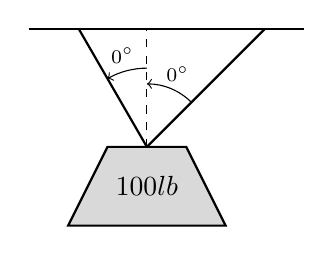
\begin{tikzpicture}
      \filldraw[thick,black,fill=gray!30] (-.5,0) -- (.5,0) -- (1,-1) -- (-1,-1)--cycle;
      \draw (0,-.5) node {$100\unit{lb}$};
      
      \draw [thick] (-1.5,1.5) -- (2,1.5);
      \clip (-1.5,1.5) rectangle (2,-1.25);
      \draw [thick,rotate=120] (0,0) -- (3,0);
      \draw [thick,rotate=45] (0,0) -- (3,0);
      \draw [dashed] (0,0) -- (0,2);
      \draw [rotate=45,->] (.8,0) arc (0:45:.8);
      \draw [rotate=67] (1,0) node {\scriptsize $0^\circ$};
      \draw [rotate=90,->] (1,0) arc (0:30:1);
      \draw [rotate=105] (1.2,0) node {\scriptsize $0^\circ$};
    \end{tikzpicture}
  \end{image}
  Find the magnitude of the force applied to each chain.
\begin{prompt}
  \[
  \text{Magnitude of the force on the left chain} = \answer{50}\unit{lb}
  \]
  \[
  \text{Magnitude of the force on the right chain} = \answer{50}\unit{lb}
  \]
\end{prompt}

\end{exercise}
\end{document}
